\documentclass[11pt]{article}
\usepackage[T1]{fontenc}
\usepackage{lmodern,microtype,amsmath,amssymb,amsthm,mathtools,booktabs,enumitem,xurl,tikz}
\usepackage[a4paper,margin=28mm]{geometry}
\usetikzlibrary{arrows.meta,positioning,calc}
\usepackage[colorlinks=true,linkcolor=blue!50!black,citecolor=blue!50!black,urlcolor=blue!50!black]{hyperref}
\setlength{\emergencystretch}{2em}
\numberwithin{equation}{section}
\newtheorem{theorem}{Theorem}[section]
\newtheorem{proposition}[theorem]{Proposition}
\newtheorem{lemma}[theorem]{Lemma}
\newtheorem{corollary}[theorem]{Corollary}
\theoremstyle{definition}\newtheorem{definition}[theorem]{Definition}
\theoremstyle{remark}\newtheorem{remark}[theorem]{Remark}
\newcommand{\ii}{\mathrm i}
\newcommand{\dd}{\,\mathrm d}
\newcommand{\RR}{\mathbb R}
\newcommand{\CC}{\mathbb C}
\newcommand{\ZZ}{\mathbb Z}
\newcommand{\T}{\mathsf T}
\newcommand{\HH}{\mathcal H}
\newcommand{\A}{\mathcal A}
\newcommand{\arccot}{\operatorname{arccot}}
\newcommand{\eps}{\varepsilon}
\title{Stationary profiles of strict Newton trees}
\author{}\date{}
\begin{document}\maketitle
\begin{abstract}
The Newton evaluation of a finite Conway expression is a sum over
integer labels on a tree. We characterize its exact positive support
and its strict real states for arbitrary ordered products and turns.
After adjacent product vertices are contracted, strictness is
equivalent to having at most one turned leaf at each remaining
vertex. The original wire lattice is primitive. A direct boundary
argument proves that its complete positive action has a unique
interior maximum, with negative definite Hessian, also on every
admissible fixed-output slice.

We determine the stationary boundary profiles and their additive
constants. The profiles of the two one-sided output types differ
from the elementary profile only by intrinsic satellite actions;
their parameters obey an exact harmonic addition law. At every
closed strict maximum the original leaf indices are at least one
quarter. These statements retain the original integer support and
the complete positive action, providing the variational data for
separate source estimates and marked geometric constructions.
\end{abstract}

\section{Introduction and exact inputs}
The boundary of a recursively constructed tangle need not behave
like the boundary of a completed pair of elementary pieces. A turn
can produce an output whose allowable indices occupy only the upper
half of the interval. Such a piece can still be attached to a lower
or unrestricted output, and the resulting closed expression can
have a strict stationary state. This paper follows the actual
integer supports through those operations and studies their
stationary profiles.

The underlying finite calculus is the Newton calculus of
\cite{Newton}. We use its multiplication, turn, circle and closure
identities, which hold in the full polynomial quotient, including
the first derivatives at repeated spectral roots. We extend its
variational argument from completed/completed roots to all strict
ordered expressions. In particular, we give the endpoint descent
and angle-map arguments on the enlarged syntax; interior existence
is not inferred from a negative Hessian.

The main finite and variational results are
Theorems~\ref{st:reduced-junctions} and \ref{st:positive-action}.
Theorems~\ref{st:profiles} and \ref{st:probe} determine the
absolute boundary profiles. Theorem~\ref{st:quarter} places every
closed stationary leaf in $[1/4,1/2)$.
The elementary positive-sum limit in
Theorem~\ref{st:positive-action} identifies that maximum with the
rate of the original positive evaluation. All expressions and their
number of leaves are fixed before $N\to\infty$.

The analytic action below is a sum of elementary ideal-tetrahedron
volume functions. Its concavity is the familiar angle-variable
calculus discussed in \cite{FuterGueritaud}; we give the derivatives
and the required boundary proof explicitly. The tangle convention
is the ordered convention of \cite{Newton}, within the usual
framework of Conway composition \cite{KauffmanLambropoulou}.
No classification up to arbitrary tangle isotopy is needed.

\subsection{The original expressions}
Each occurrence of $h$ is a distinct turned auxiliary circle around
two main strands. In a stack $FG$, $F$ lies below $G$.
The endpoints, in cyclic order, are bottom left, bottom right, top
right and top left; the exposed tuple after stacking is
$(F_0,F_1,G_2,G_3)$, with joins $F_2G_1,F_3G_0$.
The clockwise turn $\T$ sends the exposed tuple to
$(F_1,F_2,F_3,F_0)$. Cylindrical closure $C(FG)$ joins bottom to top
on both sides. The arbitrary open syntax considered here is
\[
 E::=h\mid \T E\mid E_1E_2.
\]
The original expression retains this order and every written leaf.
Algebraic regroupings below compute its source; they do not discard
physical circles or assert new isotopies.

Fix $N\ge2$, and set
\[
 d=N-1,\quad M=\lfloor d/2\rfloor,\quad q=e^{\pi\ii/N},
 \qquad S_r=\prod_{a=1}^r2\sin(\pi a/N),\quad S_0=1.
\]
Let $\mathsf C_N$ be the Chebyshev polynomial characterized by
$\mathsf C_N(\cos t)=\cos Nt$. The full pair algebra is
\[
 \HH_N=\CC[z]/(P_N(z)),\qquad P_N(z)=2\mathsf C_N(z/2)+2.
\]
Its normalized Newton basis is
\[
 e_r(z)=S_r^{-2}\prod_{a=0}^{r-1}(c_a-z),\qquad
 c_a=2\cos((2a+1)\pi/N),\quad 0\le r\le d.
\]
The nodes $c_a$ repeat, except for one simple node at odd level.
Equality in $\HH_N$ includes the first derivatives at the double
nodes.

\begin{proposition}[Imported finite calculus]\label{st:imports}
In this basis the actual turn, marked closure $\phi$ and
multiplication satisfy
\begin{align}
 \T e_r&=e_{d-r},&
 \phi(e_i e_j)&=\mathbf1_{i+j=d},\label{st:pairing}\\
 e_i e_j&=\sum_{r=\max(i,j)}^{i+j}\mu_N(i,j,r)e_r
 &&(i+j\le d),\notag\\
 \mu_N(i,j,r)&=
 \frac{S_{i+j}S_r}{S_iS_jS_{r-i}S_{r-j}S_{i+j-r}}>0,
 & e_i e_j&=0\quad(i+j>d).\label{st:product}
\end{align}
The complete pure leaf is
\begin{equation}\label{st:leaf}
 h_N=\sum_{r=0}^M a_{N,r}e_r,\qquad
 a_{N,r}=\frac{N^2S_{2r}}{S_r^4}>0.
\end{equation}
These are \cite[Proposition 3.2, Theorem 3.3, Proposition 4.1 and
equation (4.3)]{Newton}. They use the original marked normalization.
\end{proposition}
For later colored expressions, write
$L_j=(-1)^{j-1}U_{j-1}(z/2)$, where $U_n$ is the
second-kind Chebyshev polynomial,
$U_0=1$, $U_1(z/2)=z$ and
$U_{n+1}(z/2)=zU_n(z/2)-U_{n-1}(z/2)$.
It is the actual circle operator of color $j$.
The actual positive crossing in the pair algebra is
\[
 R=\kappa\sum_{r=0}^d(-q)^r e_r,\qquad \kappa=q^{d^2/2},
\]
by \cite[equation (4.8)]{Newton}; its inverse is the
negative crossing. Thus an independently colored
leaf with retained sign $\eps$ means exactly
$h_j^\eps=\T(R^\eps L_j)$. These definitions retain
the physical colors and signs in the exact rerooting identities below.
The positive source $Z_N^0$ is the scalar obtained from a fixed
$C(FG)$ by these rules with every leaf equal to $h_N$.
Its closing product has the exact coefficient-one relation
$i+j=d$. We delete that forced gate only after imposing the
relation. All other products remain.

\section{Exact supports and reduced product junctions}\label{st:syntax}
A support is a set of Newton indices with nonzero coefficients.
For the complete pure source these coefficients are nonnegative,
so supports can be computed without cancellations.

\begin{proposition}[Integer supports]\label{st:finite-support}
Every nonempty open complete support is an integer interval. If
$I_E=[l_E,u_E]\cap\ZZ$, then
\begin{align}
 I_h&=[0,M]\cap\ZZ,&
 I_{\T E}&=[d-u_E,d-l_E]\cap\ZZ,\notag\\
 I_{FG}&=
 \begin{cases}
 \varnothing,&l_F+l_G>d,\\
 [\max(l_F,l_G),\min(d,u_F+u_G)]\cap\ZZ,&l_F+l_G\le d.
 \end{cases}\label{st:interval}
\end{align}
Every coefficient in the displayed nonempty interval is positive.
An empty support remains empty under subsequent operations.
\end{proposition}
\begin{proof}
Only the product requires proof. For a proposed output $r$, the
allowable inputs lie in
$[l_F,\min(u_F,r)]$ and $[l_G,\min(u_G,r)]$.
Their sums fill an integer interval with lower endpoint $l_F+l_G$
and upper endpoint $\min(u_F,r)+\min(u_G,r)\ge r$.
Both $r$ and the lower endpoint are at most $d$, so this sum
interval meets $[r,d]$. Formula~\eqref{st:product} supplies a
positive summand. The same formula gives every necessary
inequality and the zero case.
\end{proof}
In particular
\[
 \phi(FG)=\sum_{r=0}^d [e_r]F\,[e_{d-r}]G.
\]
This identity also holds for arbitrary signed leaf coefficients.
Only the positive-support conclusion uses positivity.

\subsection{Strict real supports}
Scale the finite wire labels by $d$. A strict leaf label is
$0<a<1/2$. A strict retained product with inputs $x,y$ and output
$z$ satisfies
\begin{equation}\label{st:strict-gate}
 \max(x,y)<z<x+y<1.
\end{equation}
A turn sends $x$ to $1-x$. At a closed root impose $x+y=1$
instead of requiring a strict final product.

\begin{lemma}[The complete type table]\label{st:types}
The set of strictly realizable outputs of an open expression is
exactly one of
\[
 L=(0,1/2),\qquad H=(1/2,1),\qquad A=(0,1),\qquad\varnothing.
\]
The leaf has type $L$. Turn exchanges $L,H$, fixes $A$, and
preserves emptiness. Product is symmetric and has table
\[
 \begin{array}{c|ccc}
  &L&H&A\\\hline
 L&A&H&A\\
 H&H&\varnothing&H\\
 A&A&H&A
 \end{array}.
\]
The strict closed pairs are $AA,AL,AH,LH$ and their reversals.
\end{lemma}
\begin{proof}
For two low inputs and any $0<z<1$, choose both inputs in
$(z/2,\min(z,1/2))$. For an $L,A$ pair choose a sufficiently
small low input $c>0$ and the other input $z-c/2$.
Two $A$ inputs can use the first construction. A high input
forces $z>1/2$; for such $z$ choose that input $z-c/2$ and
the other input $c>0$ sufficiently small. Their sum is less
than one. Two high inputs cannot have sum less than one.
These choices prove sufficiency at every output in each stated
interval, as well as necessity. Finally, the closed condition is
$S_F\cap(1-S_G)\ne\varnothing$.
\end{proof}
\begin{definition}\label{st:strict-definition}
A cylindrical expression is \emph{strict} if it has a strict
reduced real state in this sense. This definition concerns its
original wire constraints.
\end{definition}
An empty strict type does not imply finite vanishing.
For example $\T h\,\T h$ has no strict state. At even $N$ its
support is empty, whereas at odd $N=2m+1$ its support
is the full interval $[m,d]$. Both original leaf
indices are then forced to their upper endpoint $m$,
so the contribution is boundary-only despite this
range of product outputs. Its cylindrical scalar
at output $d$ is positive. These assertions follow
from \eqref{st:interval}.

\subsection{A product with several inputs}
The symmetric tensor
$C_k(i_1,\ldots,i_k)=\phi(e_{i_1}\cdots e_{i_k})$
retains its normalization from \eqref{st:product}.
For $k=3$ its support is
\[
 i_1+i_2,\ i_1+i_3,\ i_2+i_3\le d,\qquad
 i_1+i_2+i_3\ge d.
\]
The input legs of a product gate are $x,y,1-z$ in this
symmetric notation.

\begin{lemma}[Multiple-input support]\label{st:hub-support}
For $n\ge2$ the product of basis elements with indices $i_1,\ldots,i_n$
is zero unless every pair satisfies $i_p+i_q\le d$. If all
these inequalities hold, its positive support is
\begin{equation}\label{st:many-support}
 [\max_p i_p,\min(d,\sum_p i_p)]\cap\ZZ.
\end{equation}
For fixed $0<x_p<1$, a prescribed output $z$ has a strict
resolution in any binary parenthesization precisely when
\begin{equation}\label{st:many-strict}
 x_p+x_q<1\ (p\ne q),\qquad
 \max_p x_p<z<\min(1,\sum_p x_p).
\end{equation}
A closed $k$-input product, $k\ge3$, has a strict resolution
precisely when
\begin{equation}\label{st:closed-hub}
 \sum_p x_p>1,\qquad x_p+x_q<1\quad(p\ne q).
\end{equation}
\end{lemma}
\begin{proof}
Associate a violating pair first to prove the finite zero
assertion. Otherwise split at any binary root. The lower
endpoints of the two child supports are their largest indices;
their sum is at most $d$ by the pair inequalities.
Proposition~\ref{st:finite-support} proves
\eqref{st:many-support} inductively, for this and every other
parenthesization.

For necessity in the strict statement, follow two inputs to
their first common gate. Its child labels are at least those
two input labels, and their sum is less than one. Following
outputs also gives the strict maximum and sum bounds.
For sufficiency, in a child set $S$ write
$L_S=\max_{p\in S}x_p$, $U_S=\min(1,\sum_{p\in S}x_p)$.
A nonsingleton child has output interval $(L_S,U_S)$;
a singleton has its prescribed value. Restrict the two
children to values below $z$. The lower endpoint of their
possible sum is $L_1+L_2<1$, and its upper endpoint is greater
than $z$, by \eqref{st:many-strict}. Thus their sum can be
chosen strictly between $z$ and one. If both are singletons,
their fixed sum already lies there. This gives a strict
parent gate, and induction fills its children.

For a closed product split at the removed final gate.
If both child sets have at least two inputs, their lower
endpoint sum is less than one and their upper endpoint sum
is greater than one, so their output intervals contain a
complementary pair. If one set is the singleton $x$, the
other interval contains $1-x$: its lower bound is smaller
by the pair inequalities, and its upper bound is larger
by the total-sum inequality. This proves sufficiency.
For necessity, two inputs meeting at a retained gate
have sum less than one. If their first common vertex
is the deleted closing gate, at least one branch
contains a strict product because $k\ge3$; its
output strictly exceeds the selected input. The two
selected inputs therefore still have sum less than
one. The same strict product makes the total of
the external inputs strictly larger than the two
closing outputs, whose sum is one.
For $k=2$ only that relation
remains, namely $x_1+x_2=1$.
\end{proof}

\subsection{The reduced junction tree}
Write $\mathbf J_{ij}=\mathbf1_{i+j=d}$. Raising one index of
$C_3$ by $\mathbf J$ recovers multiplication. Thus an internal
edge without a turn contracts through $\mathbf J$, while an
edge with a turn contracts through $\mathbf J\T=I$.
Contract unary chains modulo the algebraic identity $\T^2=I$,
suppress the degree-two closing vertex, and collapse every
internal edge without a turn. The result is a tree of
product vertices of valence at least three. We call these
vertices \emph{junctions}. Every remaining internal edge
has one turn. The original leaf labels are retained.
A leaf is \emph{flagged} if its incident edge has one turn:
it supplies $\T h$ rather than $h$.

\begin{theorem}[Reduced junction criterion]\label{st:reduced-junctions}
For a closed expression with $H\ge3$ leaves, the reduced
junction tree is unique under the indicated contractions.
The expression is strict if and only if each junction has
at most one flagged leaf. Its full finite source is the
contraction of the same tensors $C_k$, with all independent
leaf coefficients and repeated-root normal data retained.
\end{theorem}
\begin{proof}
The contracted components are exactly the connected components
of the internal edges without a turn, so they are uniquely
specified. Frobenius associativity identifies their tensor
with $C_k$. Lemma~\ref{st:hub-support} proves preservation of
strict feasibility at fixed external labels under every
collapse and resolution.

Two flagged leaves at a junction have labels greater than
$1/2$, contradicting \eqref{st:closed-hub}.
Conversely root at an internal edge, if one exists.
Every junction has at least two branches besides its parent.
An unflagged leaf supplies type $L$ and a flagged leaf type
$H$. Inductively an outward child product has type $H$ if
its own junction has one flagged leaf, and $A$ otherwise.
After the intervening turn its input to the parent has
type $L$ or $A$. The table of Lemma~\ref{st:types} therefore
gives exactly these claimed outgoing types. At the chosen
root edge one side is turned, leaving one of the closing
pairs $AA,AL,HA,HL$, each strict.
For a single junction, expose a leaf. With no flag the
remaining product has type $A$ and the pair is $L,A$.
With one flag expose it, giving $H,A$. The strict resolution
lemma transports the resulting state back to the literal
binary syntax.
\end{proof}
With two leaves there is no junction. The strict case has
one turn on their connecting edge and the two original leaf
labels are equal. We retain this case separately below.

\begin{figure}[ht]
\centering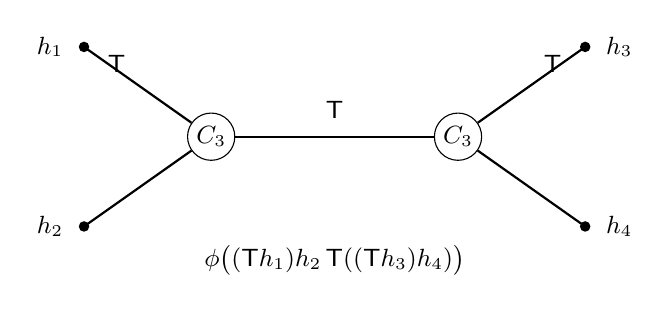
\begin{tikzpicture}[scale=.95,>=Latex,every node/.style={font=\small},
 junction/.style={circle,draw,fill=white,minimum size=6mm,inner sep=1pt}]
 \node[junction] (a) at (-1.65,0) {$C_3$};
 \node[junction] (b) at (1.65,0) {$C_3$};
 \coordinate (l1) at (-3.35,1.2);
 \coordinate (l2) at (-3.35,-1.2);
 \coordinate (l3) at (3.35,1.2);
 \coordinate (l4) at (3.35,-1.2);
 \draw[thick] (a)--(b) node[midway,above=3pt] {$\T$};
 \draw[thick] (a)--(l1) node[pos=.52,above left] {$\T$};
 \draw[thick] (a)--(l2);
 \draw[thick] (b)--(l3) node[pos=.52,above right] {$\T$};
 \draw[thick] (b)--(l4);
 \fill (l1) circle(2pt) node[left=4pt] {$h_1$};
 \fill (l2) circle(2pt) node[left=4pt] {$h_2$};
 \fill (l3) circle(2pt) node[right=4pt] {$h_3$};
 \fill (l4) circle(2pt) node[right=4pt] {$h_4$};
 \node at (0,-1.65)
 {$\phi\bigl((\T h_1)h_2\,\T((\T h_3)h_4)\bigr)$};
\end{tikzpicture}

\caption{A strict source with four original leaves. Each trivalent
vertex carries the symmetric product tensor. The middle edge has
a turn, so it is retained. A flagged leaf supplies $\T h_i$;
the other leaves supply $h_i$. Each vertex has one flagged
leaf. The labels $i$ remain independent when colors or crossings
are changed.}\label{st:tree-figure}
\end{figure}

For later estimates it is useful to record the exact outgoing
coupons. Root at a flagged leaf when one is present. A
nonroot junction gives
\begin{equation}\label{st:messages}
 Q_v=
 \begin{cases}
 \T\bigl(p_{i(v)}\prod_wQ_w\prod_lh_l\bigr),
       &\text{one flagged leaf},\\
 \T\bigl(\prod_wQ_w\prod_lh_l\bigr),
       &\text{no flagged leaf},
 \end{cases}
 \qquad p_i=\T h_i .
\end{equation}
The final scalar is $\phi(p_0\prod Q_w\prod h_l)$.
These are exact full-algebra identities, also for
$h_i=\T(R^{\eps_i}L_{j_i})$ at independent colors and signs.
The two outgoing types are respectively $L$ and $A$.
Commutativity and $\T^2=I$ in this calculation are not
claims that arbitrary physical turns or products can be
removed from the underlying tangle.

\begin{corollary}[Exposing any original leaf]\label{st:any-root}
Every original leaf of a strict closed tree with $H\ge3$
can be exposed as a closing character without changing
any other leaf. If its reduced edge parity is $\sigma$,
and $A$ is the product of the other branches at its
junction, then
\[
 Z_N=\phi((\T^\sigma h_j)A)
     =\phi(h_j\T^\sigma A)
     =\phi(p_j\T^{\sigma+1}A),\qquad p_j=\T h_j .
\]
The last factor is either an unturned product of at least
two $L/A$ branches, a decorated low module of the first
form in \eqref{st:messages}, or the turned output of an
unflagged product with at least two branches.
\end{corollary}
\begin{proof}
The pairing in \eqref{st:pairing} makes $\T$ self-adjoint:
$\phi((\T F)G)=\phi(F(\T G))$. This proves the identities.
If $\sigma=1$, the root leaf uses the only possible flag,
so all other branches are $L/A$ and
$\T^{\sigma+1}A=A$.
If $\sigma=0$ and another leaf at the junction is flagged,
$A=p_i\prod Q$ and $\T A$ is the decorated low module.
If there is no such flag, $\T A$ is the outgoing
unflagged product. The valence is at least three in
all cases. In particular an entirely unflagged
three-leaf tree is included.
\end{proof}
For a two-input product, two high Newton coordinates
vanish exactly: if $i,j>M$, then $i+j>d$ at both
parities. This finite observation is useful when the
last case of Corollary~\ref{st:any-root} has only
two inputs. It does not by itself bound a signed
character at the exposed root.

\section{The primitive polytope and its interior maximum}\label{st:variation}
For a fixed strict expression let $P$ be the compact polytope
obtained by replacing all strict leaf and product inequalities
by their weak versions. Turns retain $y=1-x$, and closure
retains the complementary relation. Its relative interior is
the strict state set: a strict state exists, so none of the
listed proper inequalities is identically an equality.

\subsection{Integer coordinates and endpoints}
\begin{lemma}[Primitive coordinates]\label{st:lattice}
A closed tree with $H$ leaves has $K=2H-3$ free integer
coordinates after the forced closing product is removed.
Every remaining finite label has the form
\begin{equation}\label{st:offsets}
 r_w=NL_w(k/N)+\delta_w,\qquad k\in\ZZ^K,
\end{equation}
where $L_w$ is integral affine and $\delta_w$ is a fixed
integer. There is no residual congruence restriction.
Every strict real state is approached by admissible states
at all sufficiently large levels of both parities.
For an open tree the full dimension is $2H-1$ and its
fixed-output slice has dimension $2H-2$.
\end{lemma}
\begin{proof}
Keep a coordinate for every leaf output and every product
output. A unary turn simply replaces its input by $d-r$.
The closed tree has $H-2$ retained products, in addition
to its $H$ leaves. Its two root subtrees are disjoint,
so the closing relation can be solved for an output
coordinate in one subtree with coefficient $1$ or $-1$.
No identification of the two root coordinates has been
made. In particular, this procedure never creates $2r=d$.
This proves the dimension and primitivity assertions.
Replacing $d$ by $N-1$ gives \eqref{st:offsets}.

Round $d$ times the free coordinates of a strict state,
and reconstruct the eliminated coordinate exactly.
The errors in all labels are bounded for the fixed
expression. Every proper inequality has a positive
slack times $d$, so the rounded state is admissible
for all sufficiently large $N$. The strict leaf slack
also puts its labels below $M$, at either parity.
For a prescribed open output $r_N/d\to b$ in the actual
strict interval, choose strict states continuously
near $b$, fix that output first and round the other
coordinates. Such a continuous choice is obtained by
interpolating two nearby strict states with output
on either side of $b$.
\end{proof}

Define
\begin{align}
 J(t)&=\int_0^t\log(2\sin\pi u)\dd u,\qquad 0\le t\le1,
       \label{st:J}\\
 g(a)&=J(2a)-4J(a)
       =-2J(a)-2J(1/2-a),\label{st:g}\\
 m(x,y,z)&=J(x+y)+J(z)-J(x)-J(y)\notag\\
 &\hspace{11mm}-J(z-x)-J(z-y)-J(x+y-z).
       \label{st:m}
\end{align}
Here $J$ has its continuous endpoint values,
$J(1-t)=-J(t)$ and $J(1/2)=0$.
The complete action is the sum of one $g$ for each
original leaf and one $m$ for each retained product:
\begin{equation}\label{st:action}
 \A(y)=\sum_{\ell=1}^H g(a_\ell(y))
             +\sum_{v=1}^{H-2}m(x_v(y),y_v(y),z_v(y)).
\end{equation}
For an open expression the sum contains all its products.

The uniform factorial estimate
\cite[Lemma 5.2]{Newton} is
$\log S_r=NJ(r/N)+O(\log N)$ for $0\le r<N$.
Applied to \eqref{st:product} and \eqref{st:leaf}, it gives
\begin{equation}\label{st:weight-rate}
 \log w_N(\mathbf r)=N\A(\mathbf r/d)+O_E(\log N)
\end{equation}
uniformly on all nonzero positive states of a fixed
expression. In using this estimate at the endpoints,
the modulus of continuity of $J$ is
$O(\eta|\log\eta|)$. Thus the changes from $r/N$ to
$r/d$, and from $M/N$ to $1/2$, contribute
$O_E(\log N)$, even at the support boundary.

\subsection{The atoms and their boundary derivative}
For $a+b+c=1$ set
\[
 V(a,b,c)=-\pi\{J(a)+J(b)+J(c)\}.
\]
This is a nonnegative function, zero on the boundary of
the angle simplex and positive in its interior.
Only these elementary properties and its derivatives
are used here. With $c=1-a-b$ its Hessian has entries
\[
 -\pi^2
 \begin{pmatrix}
  \cot\pi a+\cot\pi c&\cot\pi c\\
  \cot\pi c&\cot\pi b+\cot\pi c
 \end{pmatrix}.
\]
Both displayed diagonal sums are positive, and the
determinant is $\pi^4$, since
$\cot\pi a\cot\pi b+\cot\pi b\cot\pi c+
\cot\pi c\cot\pi a=1$. The Hessian is therefore negative
definite at a positive triple.

At a product put
\[
 p=z-x,\quad q_0=z-y,\quad r=x+y-z,\quad w=1-x-y.
\]
The subscript on $q_0$ distinguishes this angle from
the root of unity. Direct substitution gives
\begin{align}
 \pi g(a)&=2V(a,1/2-a,1/2),\label{st:leaf-atoms}\\
 \pi m(x,y,z)&=
 V(y,x,w)+V(p,q_0,2r+w)+V(p+q_0,r,r+w).
 \label{st:gate-atoms}
\end{align}
All three entries of each atom are nonnegative and sum
to one on the original gate support. Consequently the
whole action is concave on its shared-label polytope.

There are two different kinds of flat atom. At
$(0,a,1-a)$ with $0<a<1$, the directional derivative
toward a positive atom is $+\infty$:
$-J(t)=-t\log t+O(t)$ near zero.
At $(0,0,1)$ the singularities cancel. More explicitly,
along the segment with small entries $t\alpha,t\beta$,
\[
 V(t\alpha,t\beta,1-t(\alpha+\beta))
 =\pi t\{(\alpha+\beta)\log(\alpha+\beta)
                  -\alpha\log\alpha-\beta\log\beta\}
       +O(t^2).
\]
The derivative is finite. A positive atom also has a
finite derivative. Thus no atom contributes $-\infty$
along a segment toward a strict state.

\begin{lemma}[Endpoint descent]\label{st:barrier}
At every nonstrict point of a nonempty strict closed
polytope, or of an open fixed-output slice with output
in its strict interval, at least one atom in
\eqref{st:leaf-atoms}--\eqref{st:gate-atoms} is flat
but is not a vertex of its angle simplex.
\end{lemma}
\begin{proof}
First suppose a proper wire has value zero or one.
A turn replaces it by its complementary endpoint.
At a product with output zero both inputs are zero.
At a product with output one the inputs sum to one:
if both are interior, the first atom is $(y,x,0)$,
as required; otherwise one may descend to an endpoint
child. Repeating this descent in the finite tree
terminates at a leaf endpoint. A leaf of value zero
has atom $(0,1/2,1/2)$; a leaf cannot have value one.
The same argument applies to either child of the
deleted root: one descends inside that child, without
putting the removed flat gate back.

Suppose now that every wire is in $(0,1)$.
A leaf at its allowed upper endpoint $1/2$ gives
$(1/2,0,1/2)$. If every leaf is strict, a nonstrict
state must lie on a retained gate face.
When $w=0$, the first atom $(y,x,0)$ is nonvertex-flat.
When $r=0$, the third atom is $(z,0,1-z)$.
When $p=0$ and $q_0>0$, the second atom has one zero
entry and two positive entries; the case $q_0=0<p$
is symmetric. In the remaining intersection
$p=q_0=0$, one has $x=y=z\in(0,1)$ and the third
atom is $(0,x,1-x)$. This lists every gate boundary.

For a fixed-output slice the output itself is in
$(0,1)$, and the same descent applies to each proper
endpoint wire. The segment used below keeps that
output fixed. No boundary caused only by imposing
the output is included among these proper faces.
\end{proof}

\begin{theorem}[Unique strict optimizer]\label{st:positive-action}
Every strict closed expression has a unique maximizer
$y_*$ of its complete action. It is strict and its
Hessian in the primitive coordinates is negative
definite. The positive scalar satisfies the all-level
limit
\begin{equation}\label{st:positive-limit}
 \lim_{N\to\infty}\frac1N\log Z_N^0=F_0,\qquad
 F_0=\A(y_*)>0 .
\end{equation}
For an open expression of nonempty type, each output
$b$ in its strict interval has a unique strict
fixed-output maximizer. The profile
\[
 f_E(b)=\max_{\text{output }b}\A_E
\]
is real analytic and strictly concave on that interval.
It has a continuous extension to the closed feasible
output interval.
\end{theorem}
\begin{proof}
Compactness gives a maximizer. Join a nonstrict point
to a strict state in the same polytope. By
Lemma~\ref{st:barrier}, one atom contributes $+\infty$
to the one-sided derivative, and none contributes
$-\infty$. Hence the action increases and the point
cannot maximize.

At a strict product the gate Hessian is already
negative definite in $(x,y,z)$. Indeed the first
atom in \eqref{st:gate-atoms} detects
$(\delta x,\delta y)$; if those vanish, the second
detects $\delta z$. Its third atom is nonpositive
and cannot cancel either negative term.
The leaf Hessian is strictly negative since
\[
 g'(a)=2\log\cot\pi a,\qquad
 g''(a)=-\frac{4\pi}{\sin2\pi a}<0 .
\]
If all atom variations vanish, every leaf output
and retained product output is fixed. Turns then
fix their output wires, and the closing relation
fixes the eliminated coordinate. Thus the sum is
negative definite on the primitive tangent space.
This proves uniqueness by concavity.

For an open expression the same argument applies
including its output coordinate: its last product
detects that coordinate, or the expression is a
turned leaf and its leaf detects it. On a fixed-output
slice, the internal Hessian is therefore invertible.
The analytic implicit-function theorem gives a
real analytic maximizing state and profile.
The full negative Hessian has a negative Schur
complement in the output coordinate, so $f_E''<0$.
For the single-leaf case this is the displayed
formula and its reflection.

Continuity at a feasible endpoint is worth recording.
For any endpoint maximizing state, interpolate it
with an interior strict state. This supplies states
at every nearby interior output, and their actions
converge to the endpoint maximum. Conversely, every
sequence of maximizing states has a convergent
subsequence in the compact full polytope; its limit
is feasible at the endpoint. These two observations
prove continuity. They do not require finite support
at the exact endpoint for every parity.

There are at most $N^K$ positive states.
Equation~\eqref{st:weight-rate} gives the upper
limit in \eqref{st:positive-limit}. Primitive
rounding of $y_*$ gives a genuine positive summand
at every sufficiently large $N$ and the matching
lower limit. The strict leaf atoms are positive,
so $F_0>0$.
\end{proof}

\begin{lemma}[Gate curvature without leaf curvature]\label{st:gate-curvature}
For a closed strict tree with $H\ge3$, the sum of the
retained gate Hessians is itself negative definite
in the primitive coordinates.
\end{lemma}
\begin{proof}
Contract unary turn chains. Every wire in a nontrivial
root subtree appears at a retained product, either
as an input or as an output. If all gate variations
vanish, these wires have zero variation. The only
possible uncovered root subtree is a single leaf
with turns; its variation is fixed by the complementary
root relation and the other subtree. Both subtrees
can be single leaves only when $H=2$. The injectivity
and the strict gate Hessian proved above give the result.
\end{proof}

\section{Stationary boundary profiles and their constants}\label{st:profile-section}
The derivative of a fixed-output profile describes how the
maximum changes when the output moves. It is convenient to
record this derivative together with the output itself.
For a strict open output $b$, define
\begin{equation}\label{st:port}
 B=\cot\pi b,\qquad \kappa_E=e^{-f_E'(b)},\qquad
 X=\sqrt{\frac{1+B^2}{1+\kappa_E}},\qquad
 Y=\sqrt{\kappa_E}\,X .
\end{equation}
The square roots are positive. Thus
$X^2+Y^2-B^2=1$ and $f_E'(b)=2\log(X/Y)$.
We call $(B,X,Y)$ the stationary boundary parameters.
Their definitions are variational; no global geometric
realization is assumed.

\begin{lemma}[The stationary product]\label{st:port-product}
At a strict stationary product the two children and the
output have the same $X$. With child cotangents $B_1,B_2$,
\begin{equation}\label{st:port-product-equations}
 S=B_1+B_2>0,\qquad
 B_o=\frac{B_1B_2+X^2-1}{S},\qquad
 Y_o=\frac{Y_1Y_2}{S}.
\end{equation}
A turn sends $(B,X,Y)$ to $(-B,Y,X)$.
\end{lemma}
\begin{proof}
At inputs $x,y$ and output $z$, stationarity gives
$f_1'(x)=-m_x$, $f_2'(y)=-m_y$ and $f_o'(z)=m_z$.
Differentiating \eqref{st:m} yields
\begin{align*}
 e^{m_x}&=\frac{\sin\pi(x+y)\sin\pi(z-x)}
                  {\sin\pi x\sin\pi(x+y-z)},\\
 e^{m_y}&=\frac{\sin\pi(x+y)\sin\pi(z-y)}
                  {\sin\pi y\sin\pi(x+y-z)},\\
 e^{-m_z}&=\frac{\sin\pi(z-x)\sin\pi(z-y)}
                  {\sin\pi z\sin\pi(x+y-z)}.
\end{align*}
Set $D=1-B_1B_2+B_o(B_1+B_2)$. The identities
\[
 S=\frac{\sin\pi(x+y)}{\sin\pi x\sin\pi y}>0,\qquad
 D=\frac{\sin\pi(x+y-z)}
          {\sin\pi x\sin\pi y\sin\pi z}>0
\]
and \eqref{st:port} give
\[
 X_1^2=X_2^2=X_o^2=D,\quad
 Y_1^2=S(B_1-B_o),\quad Y_2^2=S(B_2-B_o),\quad
 Y_o^2=(B_1-B_o)(B_2-B_o).
\]
Taking positive roots proves the product formulas.
For a turn $f_{\T E}(b)=f_E(1-b)$, so its derivative
changes sign and its cotangent changes sign. This
proves the last assertion.
\end{proof}

\begin{proposition}[Parameters of the three types]\label{st:port-types}
On their actual strict output intervals the parameters satisfy
\begin{equation}\label{st:parameter-table}
 \begin{array}{c|c}
 L&(B,X,Y)=(B,B,1),\quad B>0,\\
 H&(B,X,Y)=(-Y,1,Y),\quad Y>0,\\
 A&-Y<B<X.
 \end{array}
\end{equation}
Consequently there are constants $c_E$ such that
\begin{equation}\label{st:rigid-profiles}
 f_E(b)=g(b)+c_E\quad(E:L),\qquad
 f_E(b)=g(1-b)+c_E\quad(E:H).
\end{equation}
\end{proposition}
\begin{proof}
For a leaf, $g'=2\log\cot\pi b$ gives $(B,B,1)$.
The turn formula exchanges the first two rows and
preserves the inequality in the third.
Consider the products giving type $A$, whose children
have type $L$ or $A$.
If the common $X<1$, put $h_0=\sqrt{1-X^2}$ and write
\[
 B_i=h_0\cot\alpha_i,\qquad
 Y_i=h_0\csc\alpha_i,\qquad 0<\alpha_i<\pi.
\]
The low type has $\alpha_i=\arccos X$ and the
unrestricted type has $\alpha_i>\arccos X$.
The positivity of $S$ gives $\alpha_1+\alpha_2<\pi$,
and \eqref{st:port-product-equations} adds these angles.
Therefore $B_o<X$ and
$B_o+Y_o=h_0\cot((\alpha_1+\alpha_2)/2)>0$.
If $X\ge1$, each child has
$\sqrt{X^2-1}<B_i\le X$, with equality at the
upper bound allowed for type $L$.
In particular $B_o>0$, and
\[
 (X-B_1)(X-B_2)<1
\]
implies $B_o<X$ by \eqref{st:port-product-equations}.
The strict inequality holds also at $X=1$, since
each $B_i>0$.

A product giving type $H$ has one high child, with
parameters $(-u,1,u)$. Hence the common $X=1$.
Its other child, of type $L$ or $A$, has parameters
$(b,1,b)$ with $b>0$. Strictness says $b-u>0$,
and the output is
\[
 \left(-\frac{ub}{b-u},1,\frac{ub}{b-u}\right).
\]
This proves all cases of the table.
Finally the first two rows determine $f_E'$ as
the derivative of $g(b)$ or $g(1-b)$ on the
connected strict interval, giving \eqref{st:rigid-profiles}.
Their constants are computed next, without a choice
of additive normalization.
\end{proof}

\subsection{The intrinsic satellite action}
No product has type $L$. A product of type $H$ has
exactly one high child. Starting at an $L$ or $H$
output, follow turns and the unique high child of
each product. This path terminates at a unique
original leaf, the \emph{distinguished leaf}.
The other children on the path are called its
satellites, and have type $L$ or $A$.
Between successive high products the number of turns
is even. Thus the full algebra also gives
\begin{equation}\label{st:spine-source}
 E_H=(\T h_*)\prod_{j=1}^m Q_j,\qquad
 E_L=\T\left((\T h_*)\prod_{j=1}^m Q_j\right),
\end{equation}
after associating the inherited products. This
identity retains the actual polynomials; its
stationary profile is simpler than the polynomial.

For a satellite $Q$ define
\begin{equation}\label{st:Omega}
 \Omega_Q=\max_{0\le a\le1/2}\{g(a)+f_Q(a)\}.
\end{equation}
The maximum is the complete action of the literal
strict closure $C(h\,\T Q)$. The strict type of
$Q$ is $L$ or $A$, so Theorem~\ref{st:positive-action}
gives a unique strict maximizer $\beta_Q$.
Its equation is
$g'(\beta_Q)+f_Q'(\beta_Q)=0$.
Consequently the satellite has parameters
\begin{equation}\label{st:satellite-parameters}
 (B_Q,X_Q,Y_Q)=(b_Q,1,b_Q),\qquad
 b_Q=\cot\pi\beta_Q>0 .
\end{equation}
For type $L$, $\beta_Q=1/4$ and $b_Q=1$;
for type $A$, the strict inequality $B_Q<X_Q$
gives $1/4<\beta_Q<1/2$ and $0<b_Q<1$.

\begin{theorem}[Harmonic response and absolute profiles]\label{st:profiles}
For the spine \eqref{st:spine-source}, let $u_0$
be the cotangent of its distinguished original leaf.
Let $v$ be the final high output's $Y$, equivalently
the final low output's $X$. At its stationary state,
\begin{equation}\label{st:harmonic}
 \frac1{u_0}=\frac1v+\sum_{j=1}^m\frac1{b_{Q_j}},
 \qquad
 c_E=\sum_{j=1}^m\Omega_{Q_j}.
\end{equation}
In particular \eqref{st:rigid-profiles} holds with
exactly this constant. The parameters $b_{Q_j}$
depend only on the corresponding satellites.
\end{theorem}
\begin{proof}
Every high product has common $X=1$, so its satellite
is at the unique state \eqref{st:satellite-parameters}.
With high input $(-u,1,u)$ and output $(-v,1,v)$,
\eqref{st:port-product-equations} gives
\begin{equation}\label{st:one-response}
 v=\frac{ub}{b-u},\qquad
 0<u<b,\qquad \frac1u=\frac1v+\frac1b .
\end{equation}
Iteration proves the first formula. Conversely every
$v,b>0$ gives the strict branch $0<u<b$; no sign
has been lost by squaring the stationary equations.

It remains to fix the constant. Suppose the incoming
high profile is $g(1-x)+c$. Send the outgoing high
label $z$ to one. Then
$v=-\cot\pi z\to+\infty$, $u\to b$ and
$x\to1-\beta_Q$. The last gate approaches
$x+\beta_Q=z=1$. Its continuous action is zero:
in \eqref{st:m} use $J(1-\beta_Q)=-J(\beta_Q)$,
or note that all three atoms in
\eqref{st:gate-atoms} are flat.
Continuity of profiles, proved in
Theorem~\ref{st:positive-action}, gives
\[
 c_{\rm out}=c+g(\beta_Q)+f_Q(\beta_Q)=c+\Omega_Q.
\]
Turns preserve the constant and the bare leaf has
constant zero. This proves the second formula.
\end{proof}
For a low satellite, $\Omega_Q=2G_0+c_Q$ where
$G_0=g(1/4)$. The formula is an identity of optimized
actions. For example at $N=3$ the complete source has
$h=10-z$ and $\T h=z^2-1$; their product is
$10z^2-2z-8$ in
$\CC[z]/((z-1)^2(z+2))$. It is not a scalar
multiple of $\T h$: the value ratio at $-2$ is
$12$, whereas the normal ratio at $1$ is $9$.
Thus the constant profile does not suppress normal
data of the source.

\subsection{Unrestricted components and their effective range}
Replace each maximal low subtree by its profile
$g+c_i$. A remaining type-$A$ subtree has syntax
\begin{equation}\label{st:skeleton}
 A::=LL\mid\T A\mid AA\mid LA\mid AL,
\end{equation}
where $L$ here is an effective profile, not a
replacement quantum leaf. The definition of the
maximum immediately gives
\begin{equation}\label{st:constant-skeleton}
 f_A(z)=f_{A^{\rm skel}}(z)+\sum_i c_i.
\end{equation}
At an unflagged junction directed toward a parent,
the outgoing expression is $Q=\T A$ with $A=FG$
an unturned product and both children of type $L$
or $A$. Its intrinsic action is
\[
 \Omega_Q=\max_{0\le a\le1/2}
                 \{g(a)+f_A(1-a)\}.
\]
This is the action of the strict closure $C(hA)$.

\begin{theorem}[The intrinsic probe range]\label{st:probe}
At this closing maximum the unturned output has
\begin{equation}\label{st:probe-port}
 (B_A,X_A,Y_A)=(-x,x,1),\qquad \frac12\le x<1.
\end{equation}
Every effective leaf in \eqref{st:skeleton},
including the closing probe, has cotangent in
$[1/2,1)$. Equality at $1/2$ occurs only when
the entire effective closure consists of three
leaves. In every other case all these cotangents
are strictly between $1/2$ and one.

The absolute identities are
\begin{equation}\label{st:probe-constant}
 \Omega_Q=F_{\rm probe}(A^{\rm skel})+\sum_i c_i,
 \qquad F_0=\sum_j\Omega_{Q_j}
\end{equation}
for a whole reduced tree rooted at a flagged leaf,
with satellites $Q_j$ at that root.
\end{theorem}
\begin{proof}
The root condition says that the two output labels
are complementary and their profile derivatives
agree. Hence their triples are $(B,X,Y)$ and
$(-B,X,Y)$. The bare probe has $(x,x,1)$,
so \eqref{st:probe-port} holds initially with
$0<x<1$, the strict upper bound coming from
$-Y_A<B_A$.
At the last product use the identities in the
proof of Lemma~\ref{st:port-product}:
\[
 1=Y_A^2=(B_F-B_A)(B_G-B_A)
             \le(X_A-B_A)^2=4x^2 .
\]
Both factors are positive because output labels
strictly exceed the inputs. This proves $x\ge1/2$.

At the root product every child has common $X=x<1$.
Its cotangent satisfies $B_i\le X$ and, by
$B_1+B_2>0$, also $B_i>-X$.
If it is type $A$, both inequalities are strict,
so $Y_i^2=1+B_i^2-X^2<1$.
Turns exchange $X,Y$. The same argument propagates
the strict bounds $X,Y<1$ through every proper
type-$A$ descendant.
For a low child $(X,X,1)$ and another child
$(B,X,Y)$, the output bound $Y_o\le1$ implies
\begin{equation}\label{st:effective-bound}
 1+B^2-X^2\le(B+X)^2,\qquad
 1\le2X(B+X)\le4X^2.
\end{equation}
The last inequality is strict for an unrestricted
neighbor. For two low children at a proper
descendant, the first is strict because $Y_o<1$.
Thus equality is possible only at the root
product with two effective low children. It
gives the three-leaf closure and $x=1/2$ at
all three leaves. This proves the range.

The first identity in \eqref{st:probe-constant}
is \eqref{st:constant-skeleton} inside the same
maximum. For the second, write the original
root source as $\phi((\T h_0)\prod Q_j)$.
The associated open high profile is
$g(1-z)+\sum_j\Omega_{Q_j}$ by
Theorem~\ref{st:profiles}. At the closing output
$z=1$ the deleted last gate has coefficient
one and $g(0)=0$. Profile continuity identifies
its endpoint maximum with precisely the original
closed action, proving the formula.
\end{proof}

One boundary case in later coefficient estimates can
be read directly from these parameters. If the last
product is $A=LF$ with $F$ unrestricted, then
\[
 B_F=\frac1{2x}-x,\qquad Y_F=\frac1{2x},\qquad
 f_F'=2\log(2x^2),\quad f_A'=2\log x .
\]
For $1/2\le x\le2/3$ both slopes lie in
$[-2\log2,0]$. This is an exact closed parameter
range; it does not assert an estimate for the
signed source. Such estimates require its actual
coefficient arrays.

\begin{corollary}[The action budget at any exposed leaf]\label{st:root-budget}
Use Corollary~\ref{st:any-root}, with root edge parity
$\sigma$ and remaining product $A$.
If $\sigma=1$, every branch of $A$ has type $L$ or
$A$ and the original complete action is
$F_0=\sum_Q\Omega_Q$, summed over those branches.
If $\sigma=0$, then $Q=\T A$ has type $L$ or $A$
and $\Omega_Q=F_0$.
\end{corollary}
\begin{proof}
For $\sigma=1$, this is the last identity of
\eqref{st:probe-constant} at the exposed flagged
root. For $\sigma=0$, the original positive closure
is $C(hA)$, whose action is exactly
$\max_a\{g(a)+f_A(1-a)\}=\Omega_{\T A}$.
This includes the decorated case in which $A$
has one high child and $\T A$ is low.
Only the finite source is rerooted; the variational
maximum and every physical leaf are unchanged.
\end{proof}

\section{The quarter bound at the original closed maximum}
\begin{theorem}[All original leaves are at or above quarter]\label{st:quarter}
At the unique complete maximum of any strict closed
expression, every stationary port satisfies $X,Y\le1$.
Every original leaf label therefore satisfies
\begin{equation}\label{st:quarter-bound}
 \frac14\le a_\ell(y_*)<\frac12 .
\end{equation}
Along an $L/H$ spine with $m$ satellites, its
distinguished original leaf additionally satisfies
$\cot(\pi a_*)\le1/(m+1)$.
\end{theorem}
\begin{proof}
At the complementary root the two triples have
opposite $B$ and equal $X,Y$. For type $AA$ the
inequalities give $|B|<\min(X,Y)$.
Together with $X^2+Y^2-B^2=1$ this gives
$X,Y<1$. For type $AL$, the low side is
$(x,x,1)$ and the unrestricted inequality
$-1<-x$ gives $x<1$.
For type $AH$, the high side has $X=1$,
and the unrestricted side gives $Y<1$.
For type $LH$, the two explicit forms force
$X=Y=1$. These exhaust the strict closing pairs.

Descend through a product. The common $X$ is
already at most one. Every child type satisfies
$B_i\le X$, and $B_1+B_2>0$ implies
$B_i>-B_j\ge-X$. Thus
$Y_i^2=1+B_i^2-X^2\le1$.
A turn exchanges the same two bounds.
At a leaf, $X=\cot\pi a>0$, proving
\eqref{st:quarter-bound}. Finally, in
\eqref{st:harmonic} one has $v\le1$ and
$b_{Q_j}\le1$, so $1/u_0\ge m+1$.
\end{proof}
The lower endpoint is attained. In
$C(h\,\T(h^s))$, the inner $s$ original leaves
have $X=1$ and hence label $1/4$.
Indeed their product has at $X=1$ the parameters
$B=Y=1/s$, its turn has $(-1/s,1/s,1)$, and
the closing leaf has cotangent $1/s$.
Thus strictness of every angle state does not force
its original leaf labels to lie strictly above one quarter.


\section{Finite reproducibility and subsequent uses}
The paper-local program \texttt{check.py} uses only the Python
standard library. It compares multiplication in the full polynomial
quotient with the stated Newton formula in finite fields, retaining
the repeated roots. It separately enumerates integer supports,
checks the multi-input support theorem under different
parenthesizations, and verifies rational instances of the local
port and harmonic identities. The output states the finite ranges.
These checks detect coefficient and indexing errors; the all-level
support, boundary, curvature and positive-sum limit proofs are the
arguments above.

The exported variational statements require no global geometric
construction. A marked geometric application must assemble the
original cells and peripheral curves. A signed-source application must separately establish the local
coefficient asymptotics and control the complementary contributions.
A full-invariant application must also perform the original filling
transform and prove noncancellation. The constants $\Omega_Q$ are
intrinsic optimized actions; replacing a profile by an effective
leaf in Section~\ref{st:profile-section} does not replace its
quantum polynomial or its independent physical colors.

\begin{thebibliography}{9}
\bibitem{Newton}
\emph{Newton coefficients and positive sources for Conway tangles},
companion paper, \href{https://sashakolpakov.github.io/murakamis_dream/papers/newton-tangles.pdf}{published PDF}.
\bibitem{FuterGueritaud}
D. Futer and F. Gu\'eritaud,
From angled triangulations to hyperbolic structures,
in \emph{Interactions between hyperbolic geometry, quantum topology
and number theory}, Contemp. Math. \textbf{541} (2011), 159--182.
\bibitem{KauffmanLambropoulou}
L. H. Kauffman and S. Lambropoulou,
On the classification of rational tangles,
Adv. Appl. Math. \textbf{33} (2004), 199--237,
\href{https://doi.org/10.1016/j.aam.2003.06.002}{doi:10.1016/j.aam.2003.06.002}.
\end{thebibliography}
\end{document}
